\chapter{Engenharia de Software Experimental}
\label{cp:engenharia}

A Engenharia de Software Experimental busca medir e avaliar modelos e tecnologias em contextos práticos, objetivando a obtenção de um corpo de conhecimento. Porém, resultados oriundos de um único experimento não são suficientes para estabelecer tal corpo de conhecimento, de modo a determinar fatos sobre um dado fenômeno devido às mais diversas variações que podem ser introduzidas no processo experimental~\cite{Basili99, Miller:2005, Shull03}. Estudos demonstram que, para a avaliação, não basta considerar somente a técnica em questão, é preciso considerar também o contexto de sua utilização, por exemplo, o tipo de software e o ambiente de aplicação~\cite{carver2004impact}. Perante a isto, se faz necessário que dados sobre estudos independentes sejam armazenados e compartilhados.

Neste contexto, a realização de estudos experimentais surgem como uma alternativa para avaliação de técnicas em diferentes contextos, assim como, a replicação de experimentos, embora não seja trivial, também auxilia na composição de um corpo de conhecimento capaz de apoiar análises consistentes das técnicas~\cite{Shull02}.

\section{Estudos Experimentais}
O ato de experimentação consiste no centro do processo científico, a qual representa uma atividade na área de pesquisa científica e se utiliza de métodos de investigação experimental para a condução de experimentos~\cite{Travassos02}. 

Segundo \citeauthoronline{Basili99}~(\citeyear{Basili99}), a experimentação ajuda a determinar a eficácia de métodos e de teorias propostas. Somente experimentos verificam as teorias, podem explorar os fatores críticos, e dar luz ao fenômeno novo para que as teorias possam ser formuladas e corrigidas.

Como apoio, os estudos experimentais atuam como ferramentas para obtenção dos dados necessários ao longo de todo o processo de desenvolvimento de software, almejando resultados objetivos e significativos para alcançar melhorias no processo. Segundo~\citeauthoronline{Wohlin2012}~(\citeyear{Wohlin2012}), tais estudos podem ser divididos nas seguintes categorias: \textbf{pesquisa de opinião}, \textbf{estudo de caso} e \textbf{experimento controlado}.

Nesta primeira categoria -- Pesquisa de Opinião -- busca-se obter dados a respeito de uma técnica ou ferramenta específica, seja uma análise qualitativa ou quantitativa, em que a realização entrevistas ou aplicação de questionários a uma amostra capaz de representar uma determinada população, em que não são realizados quaisquer controles de execução ou medidas. Em geral, modelo é aplicado em pesquisas descritivas, explicativas ou exploratórias.

A segunda categoria -- Estudo de Caso -- tem como foco o monitoramento de atividades, projetos ou tarefas visando a observar um atributo específico, ou estabelecer relações entre alguns deles, a qual se prolonga por um determinado período de tempo. Por se tratar uma atividade observacional, o nível de controle é mais elevado do que o anterior.

Por fim, na terceira categoria -- Experimentos Controlados -- o estudo experimental tem sua execução manipulada de forma direta e sistemática, a fim de se ter controle sob todos os elementos que o compõem. Diversos objetos representativos são selecionados, os quais compõem as variáveis analisadas no estudo. Podem ser efetuados experimentos controlados em ambiente universitário, de forma a reduzir custos e riscos do que aplicá-los diretamente na indústria.

A definição sobre abordagem de estudo experimental a ser escolhida está atrelada a diversos fatores. Um dos principais consiste no nível de controle necessário para avaliar a questão investigada. Mesmo sendo possível controlar as variáveis, deve-se considerar o nível de dificuldade, custo e risco envolvidos. Adicionalmente, deve-se considerar a viabilidade de replicação da situação básica investigada. Caso não haja possibilidade, sendo o custo um fator limitante, então um experimento controlado pode não ser recomendado~\cite{kitchenham1997desmet}. 

O uso de uma taxonomia pode auxiliar a generalização de resultados experimentais. Inicialmente, a taxonomia para estudos experimentais considerava estudos \textit{in vivo} e \textit{in vitro}. Estudos experimentais \textit{in vivo} envolvem pessoas em seu ambiente, e no caso de Engenharia de Software, trata-se de experimentos executados em organizações de desenvolvimento de software durante todo o processo de desenvolvimento e sob circunstâncias reais. Estudos de caso para a monitoração de projetos, que coletam dados ao longo do desenvolvimento, são exemplos dessa categoria, dada a característica essencialmente observacional. A dificuldade de isolar e controlar influências externas dificulta a análise e a validação de hipóteses~\cite{Wohlin2012}.
Em contraponto, experimentos \textit{in vitro} são executados em laboratórios, o que permite um alto grau de controle. Quando não é possível executar a associação aleatória de participantes a diferentes tratamentos, o estudo se enquadra na categoria de \textit{quasi-experimentação}~\cite{Wohlin2012}. Em Engenharia de Software, experimentos dessa classe são normalmente executados em universidades e entre grupos selecionados de organizações de desenvolvimento de software~\cite{travassos2003contributions}.

Adicionalmente, uma extensão foi proposta por~\citeauthoronline{travassos2003contributions}~(\citeyear{travassos2003contributions}), incluindo duas outras categorias -- \textit{in virtuo} e \textit{in silico} -- para acomodar estudos experimentais realizados com o apoio de modelos computacionais. A execução de experimentos \textit{in virtuo} envolvem a interação entre os participantes e modelos computacionais da realidade. Em tais experimentos o comportamento do ambiente é modelado e representado por programas de computadores, sendo descrito por um conjunto de valores de variáveis ou predicados, com os quais o participante interage reproduzindo o comportamento do sistema. Essa categoria de experimentação tem se destacado por seu baixo custo, em comparação aos modelos anteriores e sua facilidade de aplicação em situações reais (não laboratoriais).  Entretanto, possui uma forte restrição: a qualidade do modelo computacional e, indiretamente, a sua implementação. A qualidade de um modelo está relacionada à capacidade de representar fielmente o comportamento de elementos do mundo real. Além disso, o treinamento dos participantes quanto ao uso dos recursos computacionais implementados é outro importante fator de risco~\cite{travassos2003contributions}. 

Por sua vez, o termo \textit{in silico} pode caracterizar estudos executados completamente por meio de modelos computacionais, em que ambiente, objetos e participantes têm seus comportamentos representados por modelos que simulam características relevantes em estudo. Pode-se projetar ambientes de experimentação compostos de modelos numéricos que não requerem qualquer forma de interação humana. Em relação à validade, a obtenção de um modelo que represente o comportamento do participante deve ser considerado com um dos pontos de maior dificuldade. Diversas variáveis podem influenciar tal comportamento, como experiência, seriedade, aspectos culturais, dentre outros e sua construção requer completo conhecimento sobre as variáveis envolvidas~\cite{travassos2003contributions}.

Segundo~\citeauthoronline{Travassos02}~(\citeyear{Travassos02}), somente experimentos verificam as teorias, podem explorar os fatores críticos e dar luz ao fenômeno novo para que as teorias possam ser formuladas e corrigidas. O processo experimental deve ser conduzido de modo sistemático, disciplinado, controlando a avaliação de processos e de atividades humanas.

\section{Processo de Experimentação}
\label{sect:processoexperimentacao}
A avaliação de uma relação causa-efeito pode ser realizada por meio da verificação de uma hipótese em um experimento controlado. Em sua execução, manipula-se, de modo controlado, as variáveis independentes com o objetivo de observar o efeito das mudanças sobre as variáveis dependentes. Busca-se isolar quaisquer fatores que possam interferir nas relações de causa-efeito, por meio da definição de um conjunto de variáveis independentes que mapeiam possíveis relações, no âmbito do objeto de avaliação~\cite{Garcia06}. 

Desse modo, a execução de um estudo requer uma sequência de atividades estabelecidas previamente, pelas quais seja possível conduzir um processo experimental de modo preciso e sistemático. 

\begin{figure}[!ht]
\centering
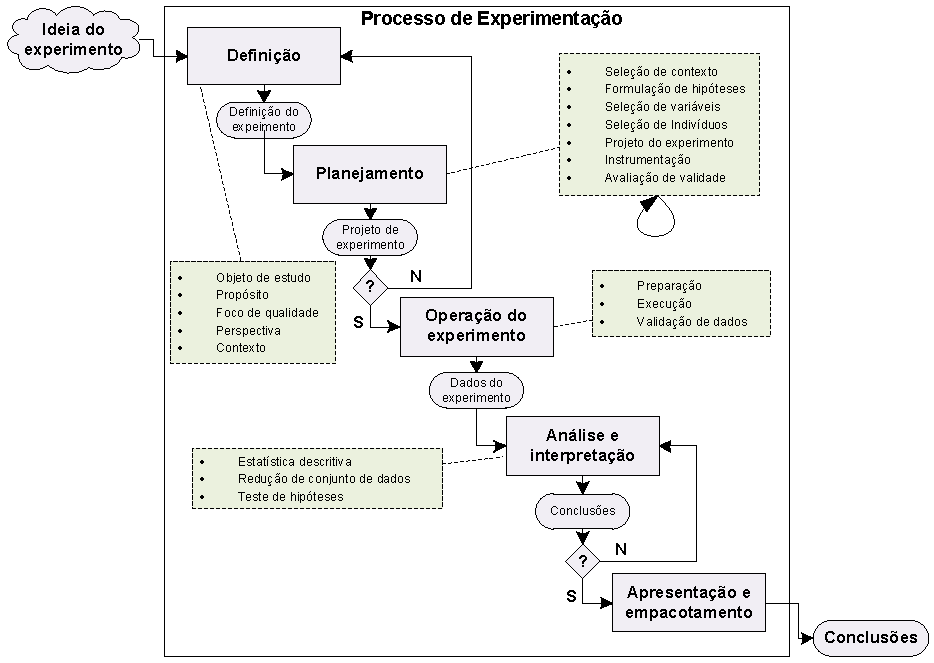
\includegraphics[width=0.98\textwidth]{images/Experimentacao.pdf}
\caption{Processo de Experimentação -- adaptado de~\citeauthoronline{Wohlin2012}~(\citeyear{Wohlin2012}).}
\label{ideia}
\end{figure}

Na Figura~\ref{ideia} é apresentado um gráfico com o processo de experimentação, adaptado de~\citeauthoronline{Wohlin2012}~(\citeyear{Wohlin2012}), é possível observar as etapas, assim como o conjunto de tarefas associado a cada uma. Cada etapa é descrita detalhadamente a seguir.


A Fase de Definição, apresentada na Figura~\ref{image:definicao}, a partir do reconhecimento de uma necessidade, é estabelecida uma sentença com a fundamentação do experimento declarando o problema a ser considerado. Deve-se estabelecer: o Objeto do Estudo (produtos, processos, recursos, etc), o Propósito (a intenção do experimento), o Foco (efetividade, custo, confiabilidade, etc), a Perspectiva (desenvolvedor, cliente, pesquisador, etc) e o Contexto (ambiente do experimento)~\cite{Garcia06}.

\begin{figure}[!htb]
\centering
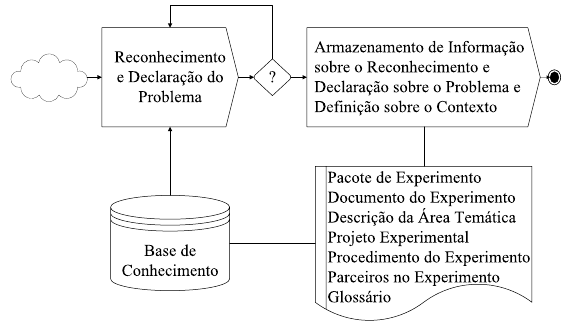
\includegraphics[width=0.7\textwidth]{images/definicao.png}
\caption{Fase de Definição~\cite{Garcia06}.}
\label{image:definicao}
\end{figure}

Em seguida, na Fase de Planejamento, descrita na Figura~\ref{image:planejamento}, deve-se determinar o Contexto de Experimentação considerando custos e riscos envolvidos, que em geral, induz à escolha de ambientes educacionais. Deve-se, também, formular as Hipóteses a serem testadas e selecionar as variáveis independentes e dependentes. A partir da Seleção dos Participantes, pode-se, então, realizar o Projeto do Experimento, elaborando o plano de condução e a submissão dos participantes aos tratamentos estabelecidos. Os métodos de análise estatística a serem aplicados aos dados devem ser estabelecidos, considerando as medidas e escalas adotadas. A elaboração do conjunto de artefatos de software, diretrizes para os participantes e questionários consiste na etapa de Instrumentação. Por exemplo, o questionário para coleta de dados relativos ao perfil de cada participante é preparado considerando as hipóteses que se deseja verificar e o mesmo se aplica a outros documentos de apoio~\cite{Garcia06}. 

Ao término dessa fase, deve ser efetuada uma análise de adequação do conjunto de dados definido, artefatos criados e elementos selecionados, e, se necessário, de modo repetido, até que se alcance a completitude necessária.

\begin{figure}[!htb]
\centering
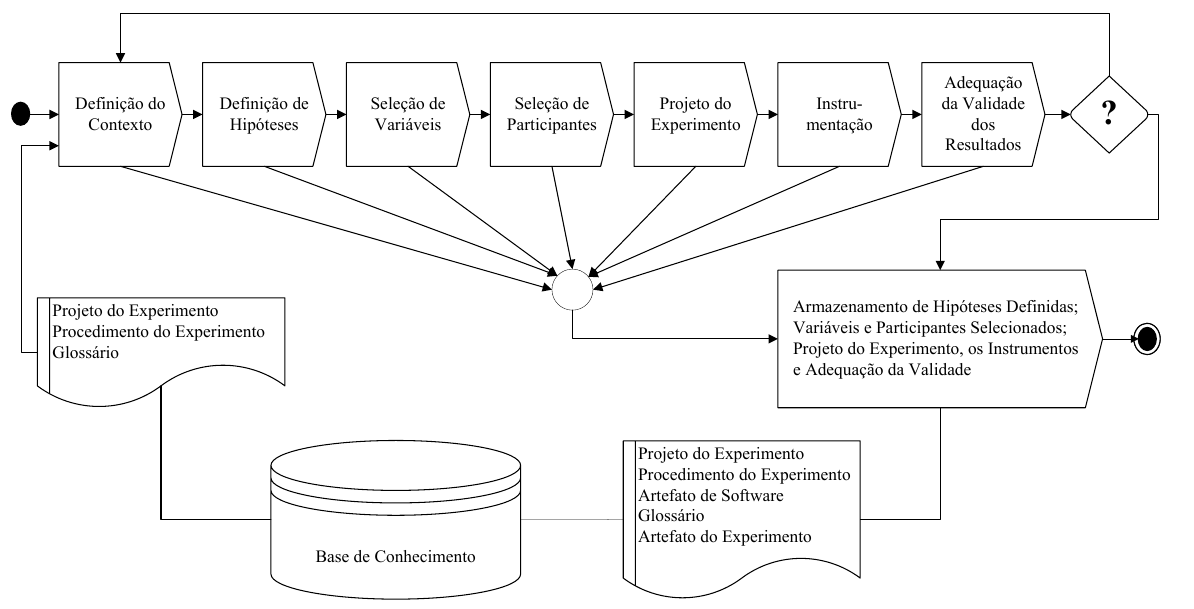
\includegraphics[width=\textwidth]{images/planejamento.png}
\caption{Fase de Planejamento~\cite{Garcia06}.}
\label{image:planejamento}
\end{figure}

A Fase de Operação, apresentada na Figura~\ref{image:operacao}, consiste na execução do experimento propriamente dita. Nessa fase, documentos gerados pelas atividades das fases anteriores, são utilizados para a condução do experimento. No final dessa fase observa-se um ponto de controle, que permite o retorno às etapas anteriores. Assim, encerra-se a execução apenas se os dados coletados forem aprovados em uma validação formal. O objetivo consiste em evitar inconsistência de dados, tais como dados incompletos, inexistentes ou incoerentes que possam dificultar a verificação das hipóteses. Vale ressaltar que, caso a coleta de dados seja apoiado por formulários eletrônicos, é possível implementar a validação dos dados, tornando desnecessário esse ponto de controle~\cite{Garcia06}. 

\begin{figure}[!htb]
\centering
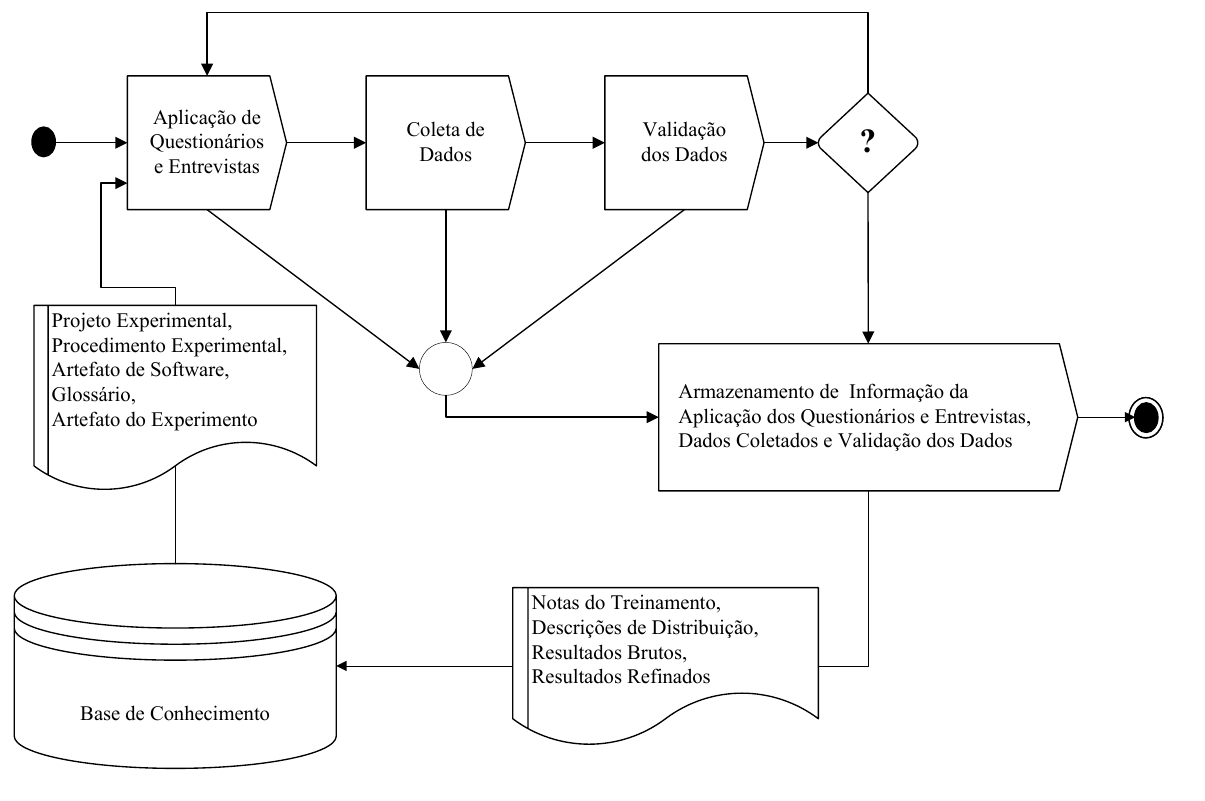
\includegraphics[width=\textwidth]{images/operacao.png}
\caption{Fase de Operação~\cite{Garcia06}.}
\label{image:operacao}
\end{figure}


Por fim, a Fase de Análise e Interpretação, representada pela Figura~\ref{image:analise} consiste em classificar os dados coletados e aplicar técnicas estatísticas, como medidas de dispersão e análise de variância. O objetivo de testar uma hipótese é verificar se é possível rejeitá-la, ou não, com base em amostra de alguma distribuição estatística, considerando uma dada margem de erro. Como os resultados dependem diretamente dos dados de entrada, o conjunto deve ser refinado e avaliado de forma a adequar-se à análise, desse modo, eliminando elementos não-confiáveis, discrepantes ou redundantes, caso existam~\cite{Garcia06}. Por fim, os dados do experimento, resultados e conclusões devem ser registrados, assim como possíveis recomendações para utilização em trabalhos futuros.

\begin{figure}[!htb]
\centering
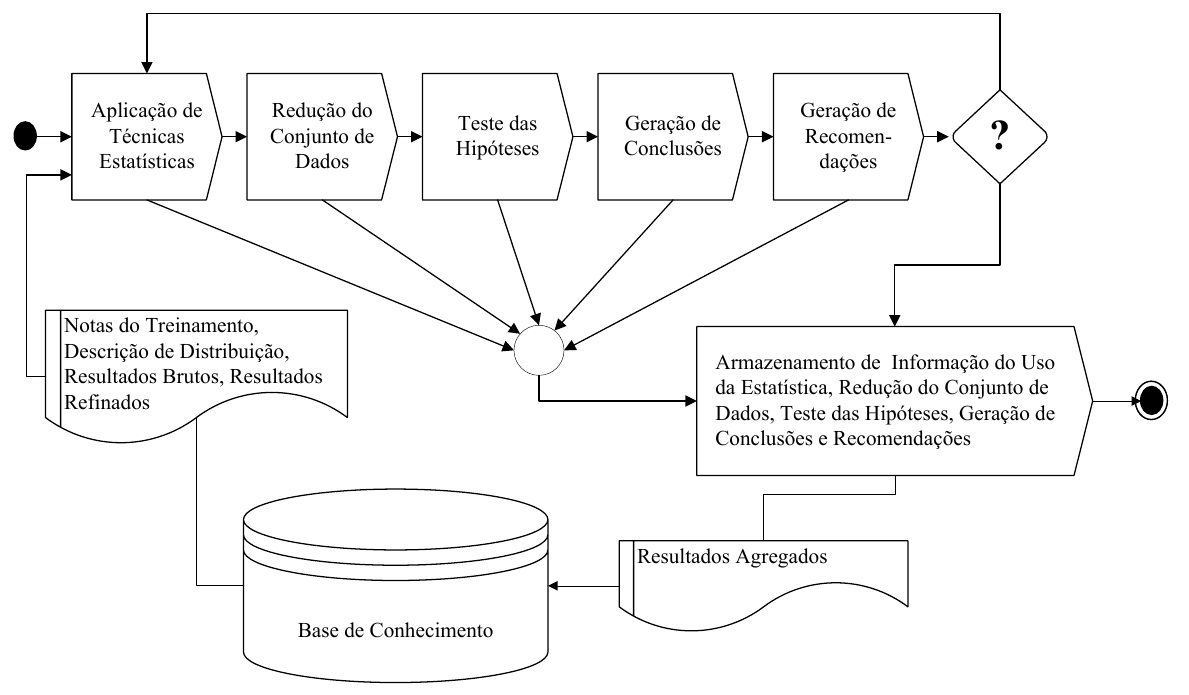
\includegraphics[width=\textwidth]{images/analise.png}
\caption{Fase de Análise e Interpretação~\cite{Garcia06}.}
\label{image:analise}
\end{figure}

Apesar de toda a relevância que um estudo experimental pode adquirir, faz-se necessária a execução em um contexto diferente, de modo a expor o dado conjunto de variáveis a fatores sociais, culturais, econômicos e tecnológicos diferentes, para solidificar o corpo de conhecimento. Tal execução pode ser realizada com a replicação do experimento.

\section{Processo de Replicação}

Segundo~\citeauthoronline{Basili99}~(\citeyear{Basili99}), a construção de um corpo de conhecimento em Engenharia de Software requer a execução de famílias de experimentos e adoção de um conjunto de princípios unificados que permita combinar e generalizar resultados. A replicação de experimentos em diferentes ambientes culturais permite não somente confirmar, ou não, hipóteses sob condições diferentes das inicialmente propostas, como também formular novos questionamentos. 

De modo a corroborar com o pensamento de que estudos isolados não são capazes de somar conhecimento,~\citeauthoronline{Miller:2005}~(\citeyear{Miller:2005}) também aponta três problemas potenciais: baixa força estatística; amplo número de potenciais influências sobre variáveis sob tratamento; e a verificação do processo e produtos do estudo.

A replicação de um experimento é de suma importância, viabiliza a análise das diferenças detectadas sob as variáveis e, consequentemente, uma avaliação com maior grau de segurança dos resultados. Além disso, a replicação permite estimar o efeito principal de qualquer fator experimental~\cite{kitchenham1997desmet}. De modo a classificar este processo,~\citeauthoronline{Basili99}~(\citeyear{Basili99}) propõem uma divisão em três categorias: 

%%
\begin{enumerate}
\item \textbf{Replicações sem variação de hipótese de pesquisa:} 
As variáveis dependentes ou independentes do experimento original não variam. Podem ser: 

\begin{itemize}
\item Replicações estritas: repetem o experimento original tão precisamente quanto possível. São necessárias para aumentar a confiança na validade da conclusão do experimento.
\item Replicações que variam a execução: variam o modo pelo qual o experimento é executado. Aumentam a confiança em resultados experimentais testando as mesmas hipóteses, mas alterando detalhes para tratar possíveis ameaças internas à validade.
\end{itemize}


\item \textbf{Replicações com variação de hipótese de pesquisa:} 
há variação de atributos do processo, produto e modelos de contexto, mas permanecem no mesmo nível de detalhamento que o experimento original. São subdivididas em: 

\begin{itemize}
\item Replicações que variam as variáveis independentes: investigam que aspectos do processo são importantes como propriedades intrínsecas, variando o processo e examinando os resultados.

\item Replicações que variam as variáveis dependentes: podem variar os modos nos quais a efetividade está sendo medida, para entender o impacto de uma tarefa em um processo pode haver melhores resultados.

\item Replicações que variam as variáveis de contexto: variação de contexto no ambiente no qual a solução é avaliada. Podem identificar fatores ambientais importantes que afetam os resultados do processo sob investigação e, assim, ajudar a entender sua validade externa.
\end{itemize}


\item Replicações de extensão teórica: objetivam determinar os limites de efetividade de um processo, aplicando grandes mudanças no processo, produto e/ou modelo de contexto, para verificar se os princípios básicos permanecem.

\end{enumerate}


Replicações de experimentos são essenciais não só para obter resultados comparativos ao experimento original, mas também para gerar e facilitar pesquisas experimentais colaborativas, transferir experiência na execução de experimentos e replicações, obter volume de dados para meta-análise e melhorar os artefatos do pacote experimental~\cite{Shull02, maldonado2006perspective}. A necessidade de conduzir um mesmo estudo em diferentes contextos para formar um corpo de conhecimento confiável introduz complicadores adicionais no processo de experimentação. Um aspecto fundamental para a condução de replicações e o uso do conhecimento nelas adquirido é o registro preciso do procedimento de condução do experimento em um Pacote de Laboratório.

\begin{figure}[!htb]
\centering
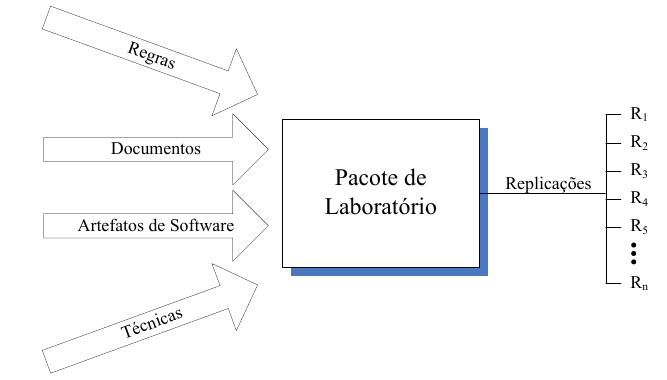
\includegraphics[width=0.9\textwidth]{images/replicacao.png}
\caption{Replicações de um experimento e o Pacote de Laboratório~\cite{Garcia06}.}
\label{image:replicacao}
\end{figure}

Na Figura~\ref{image:replicacao}, o item \textit{Regras} refere-se à condução do experimento, como distribuição de participantes em equipes e documentos, e o tempo de treinamento; o item \textit{Documentos} refere-se aos documentos utilizados para treinamento e avaliação; o item \textit{Artefatos de Software} consiste no conjunto de artefatos utilizado, por fim, o item \textit{Técnicas} refere-se não somente à técnica propriamente dita, mas também ao treinamento. Outra dificuldade encontrada diz respeito à habilidade de compartilhar conhecimento entre replicadores, que é fundamental para a execução de replicações e sua melhoria. 

Segundo~\citeauthoronline{Shull02}~(\citeyear{Shull02}), a partir da replicação de um experimento, além de verificar hipóteses, os experimentadores devem: facilitar a colaboração entre parceiros, transferir conhecimento sobre a execução do experimento e replicações, conduzir meta-análises, e melhorar o empacotamento artefatos experimentais para futuras replicações. Além disso, há a possibilidade de combinar dados de vários experimentos para a condução de análise exploratória. Nesse contexto, faltam diretrizes que apoiem o registro e manutenção de informações explícitas e no nível de granularidade adequado.

Observa-se, também, a necessidade de critérios e diretrizes para a análise de dados oriundos de replicações distintas ou com alto nível de similaridade, no processo de empacotamento, transferência de conhecimento e condução de análises exploratórias. Todos consistem problemas a serem tratados na experimentação em Engenharia de Software~\cite{Garcia06}. 


\section{Considerações Finais}
Neste capítulo foi apresentada uma sucinta definição de Engenharia de Software Experimental, demonstrando a importância de estudos experimentais em suas diferentes categorias, especialmente em relação a experimentos controlados e cada uma de suas fases no processo experimental. Vale ressaltar que embora seja elaboração um processo sistemático e controlado, tais atributos não fornecem os parâmetros necessários para a composição de um corpo de conhecimento. 
Desse modo, verifica-se a necessidade da execução de processos replicação, por exemplo, entre grupos de pesquisa, de forma a expor a execução do experimento a diferentes contextos e níveis de experiência, visando eliminar possíveis influências sob o estudo experimental. Esse aprimoramento de conhecimento a partir de diversos estudos experimentais é tratado no próximo capítulo.


